\documentclass[spanish]{beamer}
\usepackage[ansinew]{inputenc} % Acepta caracteres en castellano
\usepackage[spanish]{babel}    % silabea palabras castellanas
\usepackage{amsmath}
\usepackage{mathtools,cancel} % cancela con una flecha \cancelto{0}{XXXX}
\renewcommand{\CancelColor}{\color{red}} %change cancel color to red
\usepackage{amsfonts}
\usepackage{amssymb}
\usepackage{dsfont}
\usepackage{graphicx}
\usepackage{geometry}
\usetheme{Madrid}
\usecolortheme{beaver}
\usepackage{textpos}
% Logo  en el comienzo 
\addtobeamertemplate{frametitle}{}{%
\begin{textblock*}{100mm}(.85\textwidth,-1cm)
{\includegraphics[height=0.4in, keepaspectratio=true]{/Users/luisnunez/Dropbox/MisDocumentos/UIS/UISImagenInstitucional/UISLOGO.png}}
\end{textblock*}}

\begin{document}

\title{\textbf{Modos normales de oscilaci�n} }
\author[L.A. N��ez]{\textbf{Luis A. N��ez}}  
\institute[UIS]{\textit{Escuela de F�sica, Facultad de Ciencias, } \\
\textit{Universidad Industrial de Santander, Santander, Colombia } \\
{\includegraphics[height=0.4in, keepaspectratio=true]{/Users/luisnunez/Dropbox/MisDocumentos/UIS/UISImagenInstitucional/UISLOGO.png}}
}
\date{\today}
\maketitle


\begin{frame}
\frametitle{Agenda}
  \tableofcontents
\end{frame}


%%%%% Diapo 1
\section{Modos normales de oscilaci�n}
\frame{
  \frametitle{Modos normales de oscilaci�n 1/2}
   \begin{itemize}  
  	\item<1-> Las $s$ ecuaciones de movimiento para un sistema con peque�as oscilaciones $\left\{\eta_1, \ldots, \eta_s\right\}$ alrededor del equilibrio de $\left\{q_{01},  \ldots, q_{0 s}\right\}$ son $\sum_j\left(T_{i j} \ddot{\eta}_j+V_{i j} \eta_j\right)=0, \quad i=1,2, \ldots, s$
	\item<2-> Si suponemos una soluci�n de la forma $\eta_j(t)=a_j e^{i \omega t}$ tendremos $\sum_j\left(V_{i j}-\omega^2 T_{i j}\right) a_j=0 \quad i=1,2, \ldots, s$
	\item<3-> La condici�n $\operatorname{det}\left|V_{i j}-\omega^2 T_{i j}\right|=0 $ es decir $\left|\begin{array}{ccc}V_{11}-\omega^2 T_{11} & V_{12}-\omega^2 T_{12} & \ldots \\ V_{21}-\omega^2 T_{21} & V_{22}-\omega^2 T_{22} & \\ V_{31}-\omega^2 T_{31} & \\ \vdots & & \end{array}\right|=0$
	\item<4-> Esto permite calcular las $s$ frecuencias de peque�as oscilaciones $\omega_k, \quad k=1,2, \ldots, s$ como soluciones al polinomio caracter�stico
\end{itemize}
}
%%%%% Diapo 2
%\section{Secci�n}
\frame{
  \frametitle{Modos normales de oscilaci�n 2/2}
\begin{itemize}
	\item<1-> 	Para cada $\omega_k$, existe un sistema de $s$ ecuaciones para $a_j\left(\omega_k\right)$. \\ 
 	Si  $s=2$ \\
	$i=1:  \left(V_{11}-\omega_k^2 T_{11}\right) a_1+\left(V_{12}-\omega_k^2 T_{12}\right) a_2=0$ \\
	$i=2:  \left(V_{21}-\omega_k^2 T_{21}\right) a_1+\left(V_{22}-\omega_k^2 T_{22}\right) a_1=0$ \\ Para cada $\omega_k$ tendremos $2$ ecuaciones lineales para $a_1\left(\omega_k\right)$ y $a_2\left(\omega_k\right)$
	\item<3-> La soluci�n general, $\eta_j(t)$, ser� la superposici�n de las soluciones $\eta_j(t)=\sum_k c_k a_j\left(\omega_k\right) e^{i \omega_k t}$, donde $c_k$ son las fases complejas.
	\item<4-> Si  $\xi_k \equiv c_k e^{i \omega_k t}, \quad k=1,2, \ldots, s$, tendremos $\eta_j(t)=\sum_k a_j\left(\omega_k\right) \xi_k$ la soluci�n es una combinaci�n lineal de las coordenadas normales
	\item<5-> Cada coordenada normal $\xi_k$ satisface la ecuaci�n $\ddot{\xi}_k+\omega_k^2 \xi_k=0$.
	\item<6-> En el caso de $s=2$, las soluciones generales para los peque�os desplazamientos son $\eta_1=a_1\left(\omega_1\right) \xi_1+a_1\left(\omega_2\right) \xi_2, \quad \eta_2=a_2\left(\omega_1\right) \xi_1+a_2\left(\omega_2\right) \xi_2$
	\item<7-> Para $\xi_2$ tenemos $\eta_1=a_1\left(\omega_2\right) \xi_2, \quad \eta_2=a_2\left(\omega_2\right) \xi_2
$,  2 peque�os desplazamientos que oscilas con la frecuencia $\omega_2$ alrededor de su posici�n de equilibrio con amplitudes $a_1\left(\omega_2\right)$ y $a_2\left(\omega_2\right)$.

\end{itemize}

}
%%%%% Diapo 2
\section{Secci�n}
\frame{
\frametitle{T�tulo transparencia}
\begin{itemize}  
	\item<1-> 
\end{itemize}
}
%%%%% Diapo 2
\section{Secci�n}
\frame{
\frametitle{T�tulo transparencia}
\begin{itemize}  
	\item<1-> 
\end{itemize}
}
%%%%% Diapo 2
\section{Secci�n}
\frame{
\frametitle{T�tulo transparencia}
\begin{itemize}  
	\item<1-> 
\end{itemize}
}
%%%%% Diapo 2
\section{Secci�n}
\frame{
\frametitle{T�tulo transparencia}
\begin{itemize}  
	\item<1-> 
\end{itemize}
}  
\end{document}

\quad \Rightarrow a_j \neq 0, \forall j \quad \Leftrightarrow \omega_k, \quad k=1,2, \ldots, s

	\begin{figure}[t]
		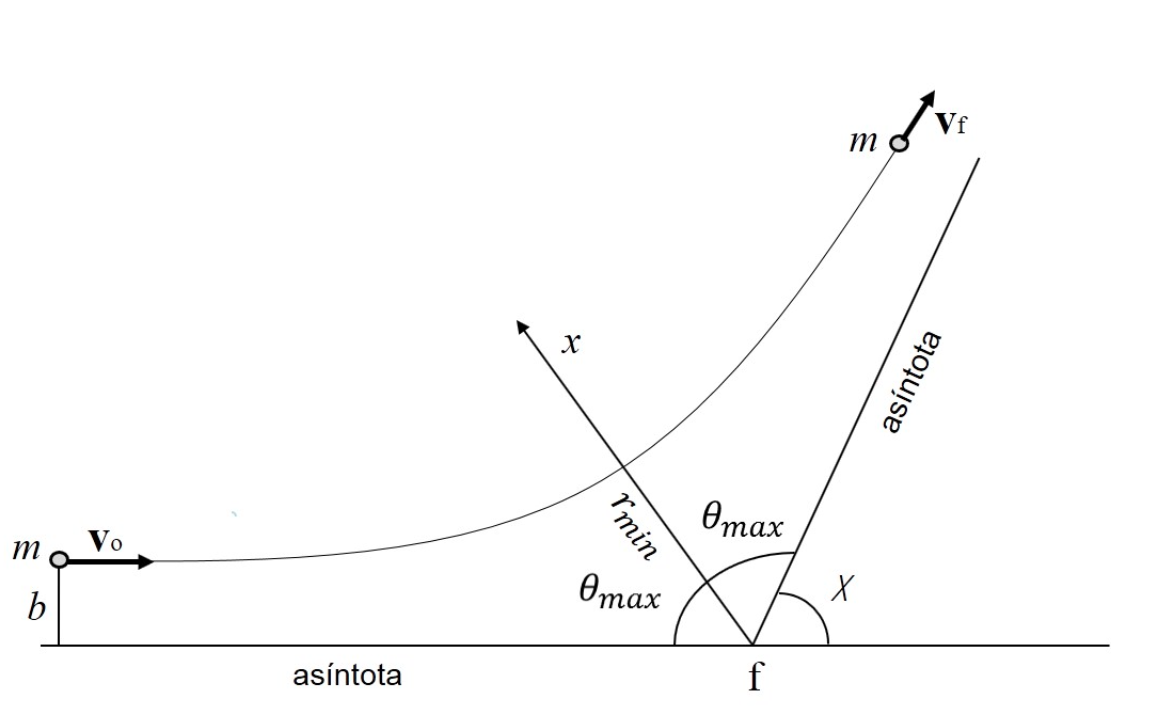
\includegraphics[width=1.8in]{Figuras/Dispersion.png}
   	\end{figure}
	
